%%
% The BIThesis Template for Bachelor Graduation Thesis
%
% 北京理工大学毕业设计(论文)第一章节 —— 使用 XeLaTeX 编译
%
% Copyright 2020-2022 BITNP
%
% This work may be distributed and/or modified under the
% conditions of the LaTeX Project Public License, either version 1.3
% of this license or (at your option) any later version.
% The latest version of this license is in
%   http://www.latex-project.org/lppl.txt
% and version 1.3 or later is part of all distributions of LaTeX
% version 2005/12/01 or later.
%
% This work has the LPPL maintenance status `maintained'.
%
% The Current Maintainer of this work is Feng Kaiyu.
%
% 第一章节

\chapter{课题简介}

本毕业设计项目,旨在对实验室的已有工作——基于Go-Ethereum实现的树状区块链——进行性能测试,验证其基于GeoHash物理位置划分子链的设计,在诸如出租车调度等需要根据节点物理位置提供不同服务的应用场景中能达成相较传统单链区块链更高的效率;同时,对其进行优化,包括:简化配置、部署区块链的流程,重构已有代码提升可维护性和可拓展性等;最后,探讨将树状区块链的基于Go语言的Go-Ethereum实现,通过Substrate工具包移植到Rust编程语言上的可能性,并进行部分移植工作以佐证之。

\chapter{当前进度}

自开题以来,笔者已经完成了数项工作,推进了毕业设计项目的整体进度。现将其陈述如下:

\section{在传统单链区块链下进行复现工作}

树状区块链的设计思想为:将原本单链结构的区块链,以类似字典树的形式,转换为树状多链结构;而在其中作为键决定某个叶子节点应该属于哪个分支的,就是叶子节点的GeoHash值。因此,笔者特地选择了需要用到GeoHash值作为索引,以在不同地区提供不同服务的应用场景——基于Dapp的出租车调度系统,作为本项目的实验场景。

在实验室的以往工作中,已经存在在单链区块链上部署并使用该系统的记录。为详细比较该系统在两种不同的区块链上的性能表现差异,笔者首先借助虚拟机,在Ubuntu 22.04系统下完成了在单链区块链上部署并使用该调度系统的工作,基本复现了实验复现手册中记载的结果,并形成了实验日志以便日后查阅。下将结合笔者复现实验的步骤,进行简要介绍。

一个去中心化的区块链网络,由数台计算机共同组成,这些计算机就称之为“节点”。为使出租车调度系统正常运行,笔者搭建了由一个节点组成的区块链网络,供后续实验之用。

首先,需要构建这个节点。

\begin{enumerate}
  \item 使用附录A中的配置文件,初始化节点;
  \item 启动节点,并指定其rpc端口为8545,以便外部程序与区块链互动;
  \item 待节点启动之后,记录其enode信息。
\end{enumerate}

一旦节点启动,终端中就会出现JavaScript控制台。此时,可以使用Go-Ethereum的官方文档中记录的各种指令,进行账户创建、解锁账户、启停挖矿、部署或调用合约等操作,与区块链进行交互。在此,笔者使用personal.newAccount("123456")新建了8个密钥均为123456的账户,一部分账号,将在出租车调度系统中承担司机与乘客的角色。

准备好区块链网络后,笔者继续完成了出租车调度系统的部署。该调度系统分为两部分,其中一部分是运行在区块链上的DApp,以智能合约的形式存在;另一部分是运行在本地浏览器中的客户端,是一套由Vue 2编写的Web GUI。本节中,笔者完成了智能合约的部署,并根据返回信息,修改了Web GUI中的部分参数,实现了系统的运行。

该系统一共需要部署两份合约。笔者将以其中一份StoreMap.sol为例,讲解合约部署的步骤。该合约为实验室已有工作的副本,存放于笔者实验的代码仓库中。使用Remix IDE在线开发环境对其进行编译后,可获得ABI(形如JavaScript的列表)和字节码(代表一个十六进制数的字符串)。将获得的上述编译结果,复制到以下部署代码中:

\begin{lstlisting}[caption={合约部署代码}]
abi = JSON.parse("压缩转义的ABI,可借助在线工具完成压缩转移步骤")
bytecode = "字符串形式的字节码"

StoreMapContract = web3.eth.contract(abi);
web3.eth.estimateGas({data: bytecode})
StoreMap = StoreMapContract.new({
    from: web3.eth.accounts[0],
    data: bytecode,
    gas: '3000000',
    position:"w2511111111111",
    txtime:277001
  },function (e, contract){
    console.log(e, contract);
    if(!e){
        if(!contract.address) {
            console.log("Contract transaction send: TransactionHash: " + contract.transactionHash + " waiting to be mined...");
        } else {
            console.log("Contract mined! Address: " + contract.address);
            console.log(contract);
        }
    }
});
\end{lstlisting}

复制到节点的JavaScript控制台中,连续按压数次回车后,使用miner.start(1)开始挖矿,注意输出,直到出现如下的合约地址:
\begin{lstlisting}[caption={挖矿输出合约地址}]
null [object Object]
Contract mined! Address: 0xef00ade84bb560afe4b562bfd4a81300c17ac52f
[object Object]
\end{lstlisting}

此时可以执行miner.stop()停止挖矿,并妥善保存好该合约的地址。

经过类似步骤,可以将另一份合约StoreTraffic.sol一同部署到区块链上,同样记录好合约地址。

合约部署结束后,按照实验室已有的手册进行操作,对客户端系统进行配置,将其中涉及到合约地址和账户公钥的代码更改为实际的合约地址和账户公钥,并上传地图文件,启动调度系统,即可观察到其运行效果。如下展示的分别是司机选择是否接单,和乘客到达目的地时系统的提示:

\begin{figure}[htbp]
  \centering
  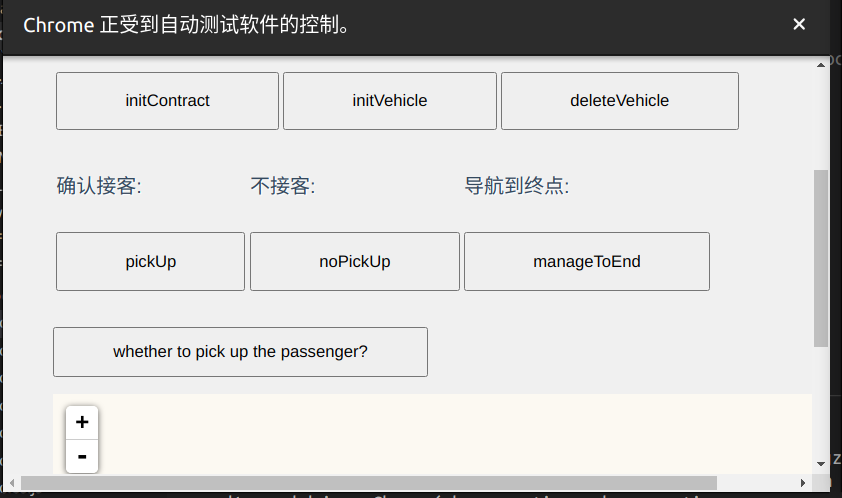
\includegraphics[width=0.9\linewidth]{images/司机接客.png}
  \caption{司机接客}\label{司机接客} % label 用来在文中索引
\end{figure}

\begin{figure}[htbp]
  \centering
  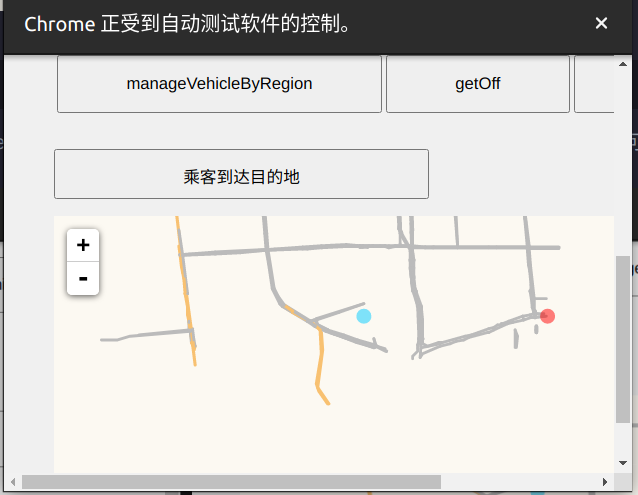
\includegraphics[width=0.9\linewidth]{images/乘客抵达.png}
  \caption{乘客抵达}\label{乘客抵达} % label 用来在文中索引
\end{figure}

\section{部分重构优化工作}

为简化树状区块链的构建流程,实验室已有使用Bash脚本等工具替代人工手动输入代码,实现树状区块链初始化、添加对等节点等操作。然而,许多实验性质的脚本并不具备可复用性,异或是在使用中出现了意想不到的异常行为。为此,笔者对已有的脚本进行了一些重构和优化,并摘取其中几例加以说明。

\subsection{对初始化并启动节点的脚本进行优化}

若令一些初始化并启动节点的脚本再运行第二次,可能导致其直接崩溃,无法启动节点。根据其报错信息,笔者断定该问题如下:每次启动节点,脚本都将调用一个JavaScript预加载脚本,以设置分支区块。然而,该设置分支区块的过程并不能重复执行,并且脚本并未对是否已设置过分支区块进行检查。综上,笔者修改了预加载脚本的内容为:

\begin{lstlisting}[caption={修改后的预加载脚本}]
// eth.setBranchBlock({from:eth.accounts[0],branchid:"w1",settime:10})  // 此行为原先的预加载脚本
if (eth.getBranchBlockByRegion("w1") === null) {
    // 若该分支区块未设置,则设置分支区块
    eth.setBranchBlock({ from: eth.accounts[0], branchid: "w1", settime: 10 })
} else {
    // 否则,执行对子叶子区块的访问操作以建立连接
    eth.getBranchBlockByRegion("w11")
    eth.getBranchBlockByRegion("w12")
}
\end{lstlisting}

经过以上改进,脚本不再崩溃,并且能够确保每次运行均能正常启动节点。

\subsection{对监控分支节点日志的脚本进行优化}

在树状区块链运行时,分支节点会持续将输出信息到日志文件中,通过读取该日志文件即可得知分支节点接收到的交易双方、交易明细等信息,再利用这些信息进行一些操作。然而,随着分支节点运行,日志内容也会不断变多,因此,需要监控该日志文件的脚本每次读取均从新增添的行开始,而非每次都从第一行读取。实验室已有的脚本并不具备该功能,笔者经过研究,最终编写出如下代码,解决了这个问题:

\begin{lstlisting}[caption={修改后的监控日志脚本}]
  "use strict";

  const fs = require('fs');
  const lineReader = require('line-reader');

  const transferjs = require("./transfer_test2");

  const filename = "../result/log_w1";
  var trans_acc = "", trans_outchain = "", trans_acc_old = "", trans_outchain_old = "";

  function main() {
      // 每次读之前都把日志文件清空
      fs.open(filename, "w", (_err, _fd) => {})

      let linePointer = -1

      fs.watchFile(
          filename,
          { persistent: true, interval: 1000 },
          (currentFileStatus, previousFileStatus) => {
              if (currentFileStatus.mtime > previousFileStatus.mtime) {
                  let tempCounter = 0
                  lineReader.eachLine(filename, (line, isLast) => {
                      if (tempCounter > linePointer) {
                          // 读取到新行,处理逻辑
                          console.log(line)

                          if (line === "--handler-TX_request--") {
                              console.log("Received handler-TX_request\n")
                          } else if (line.startsWith("***---from:")) {
                              line = line.slice(11, line.length - 6)
                              trans_acc = line.toString();
                              console.log("trans_account = " + trans_acc)
                          } else if (line.startsWith("***---outchain:")) {
                              line = line.slice(15, 29)
                              while (line[0] === 'a') {
                                  line = line.slice(1,)
                              }
                              trans_outchain = line.toString()
                              console.log("outchain(target?) = " + trans_outchain)
                              if (trans_acc != trans_acc_old && trans_outchain_old != trans_outchain) {
                                  trans_acc_old = trans_acc;
                                  trans_outchain_old = trans_outchain;
                                  transferjs.get_outchain_info(trans_acc, trans_outchain)
                              }
                          }
                      }
                      linePointer = Math.max(tempCounter, linePointer)
                      tempCounter++
                  })
                  // console.log("linePointer = ", linePointer)
              }
          }
      )
  }

  main()

  // 以下注释内容为实验室已有的日志监控脚本内容
  // fs.watchFile(fn, { persistent: true, interval: 500 },
  //     function (curr, prev) {
  //         if (curr.mtime > prev.mtime) {
  //             //文件内容有变化,那么通知相应的进程可以执行相关操作。例如读物文件写入数据库等
  //             // console.log("1--counter1:",counter1)
  //             // console.log("1--counter2:",counter2)
  //             counter1 = counter2;
  //             counter2 = 0;
  //             read_file();
  //         }
  //     }
  // )

  // //读文件
  // function read_file() {
  //     lineReader.eachLine(fn, function (line, last) {
  //         counter2++;
  //         if (counter2 > counter1) {
  //             // console.log("2--counter1:",counter1)
  //             // console.log("2--counter2:",counter2)
  //             if (line.toString() === '--handler-TX_request--') {
  //                 console.log("--get--handler-TX_request--\n")
  //             }
  //             if (line.slice(0, 11).toString() === '***---from:') {
  //                 line = line.slice(11, line.length - 6)
  //                 trans_acc = line.toString();
  //                 console.log("trans_acc:" + trans_acc)
  //             }
  //             if (line.slice(0, 15).toString() === '***---outchain:') {
  //                 line = line.slice(15, 29)
  //                 while (line.slice(0, 1).toString() === 'a') {
  //                     line = line.slice(1,)
  //                 }
  //                 trans_outchain = line.toString()
  //                 console.log("outchain:" + trans_outchain)
  //                 if (trans_acc != trans_acc_old && trans_outchain_old != trans_outchain) {
  //                     trans_acc_old = trans_acc;
  //                     trans_outchain_old = trans_outchain;
  //                     transferjs.get_outchain_info(trans_acc, trans_outchain)
  //                 }
  //             }
  //         }
  //     });
  // }

\end{lstlisting}

\section{外语文献翻译工作}

由于需要考察将基于Go-Ethereum实现的树状多链移植到Substrate上的可行性,笔者选择了翻译Substrate的英文官方文档,并完成了5000词的额定工作量。译文和对应的原文已上传至北京理工大学毕业设计管理系统。

\chapter{现有问题}

截至目前,笔者将进行工作历程中遇到的困难和挑战归结为以下几点:
\begin{enumerate}
  \item 思维模式转变不及时,未能很好地从中心化的普通网络式思维切换到去中心化的区块链式思维
  \item 对一些难度较大的工作具有畏难情绪,(例如阅读树状区块链的实现源代码),导致进度不及预期;
  \item 时间安排不够妥当,对于独立的各项事务应当并行安排工作时间,以节省总时间;
  \item 沟通不及时,和实验室中有工作内容相关的同学、前辈、老师沟通不够顺畅,导致获取、提供帮助,和同步进展不够及时;

\end{enumerate}

\chapter{后续工作}

结合目前的工作状况和待完成的任务情况,笔者如此安排日后的工作:

% 三线表
\begin{table}[htbp]
  \linespread{1.5}
  \zihao{5}
  \centering
  \caption{统计表}\label{统计表}
  \begin{tabular}{*{5}{>{\centering\arraybackslash}p{6cm}}} \toprule
    预计完成日期 & 工作内容                                         \\ \hline
    4月16日      & 完成双账号资产转移实验                           \\
    4月20日      & 完成更大规模的资产转移实验,与出租车调度系统对接,收集实验数据 \\
    4月30日      & 探究Go-Ethereum的部分实现                        \\
    5月20日      & 撰写毕业论文                                     \\ \bottomrule
  \end{tabular}
\end{table}

% \textcolor{blue}{公式标注应于该公式所在行的最右侧。对于较长的公式只可在符号处(+、-、*、/、$\leqslant$ $\geqslant$ 等)转行。在文中引用公式时,在标号前加“式”,如式(1-2)。阅后删除此
%   段。}

% \textcolor{blue}{公式-示例:(阅后删除此段)}
% % 公式上下不要空行,置于同一个段落下即可,否则上下距离会出现高度不一致的问题
% \begin{equation}
%   LRI=1\ ∕\ \sqrt{1+{\left(\frac{{\mu }_{R}}{{\mu }_{s}}\right)}^{2}{\left(\frac{{\delta }_{R}}{{\delta }_{s}}\right)}^{2}}
% \end{equation}

% 一个可能无法正常显示的生僻字
% 一个可能无法正常显示的生僻字: 彧。下文注释中,介绍了如何通过自定义字体来显示生僻字。

% 定义一个提供了生僻字的字体,注意要确保你的系统存在该字体
% \setCJKfamilyfont{custom-font}{Noto Serif CJK SC}

% 使用自己定义的字体
% 使用提供了相应字型的字体:\CJKfamily{custom-font}{彧}。

